\subsubsection{Screens Flow}

\begin{figure}[H]
    \centering
    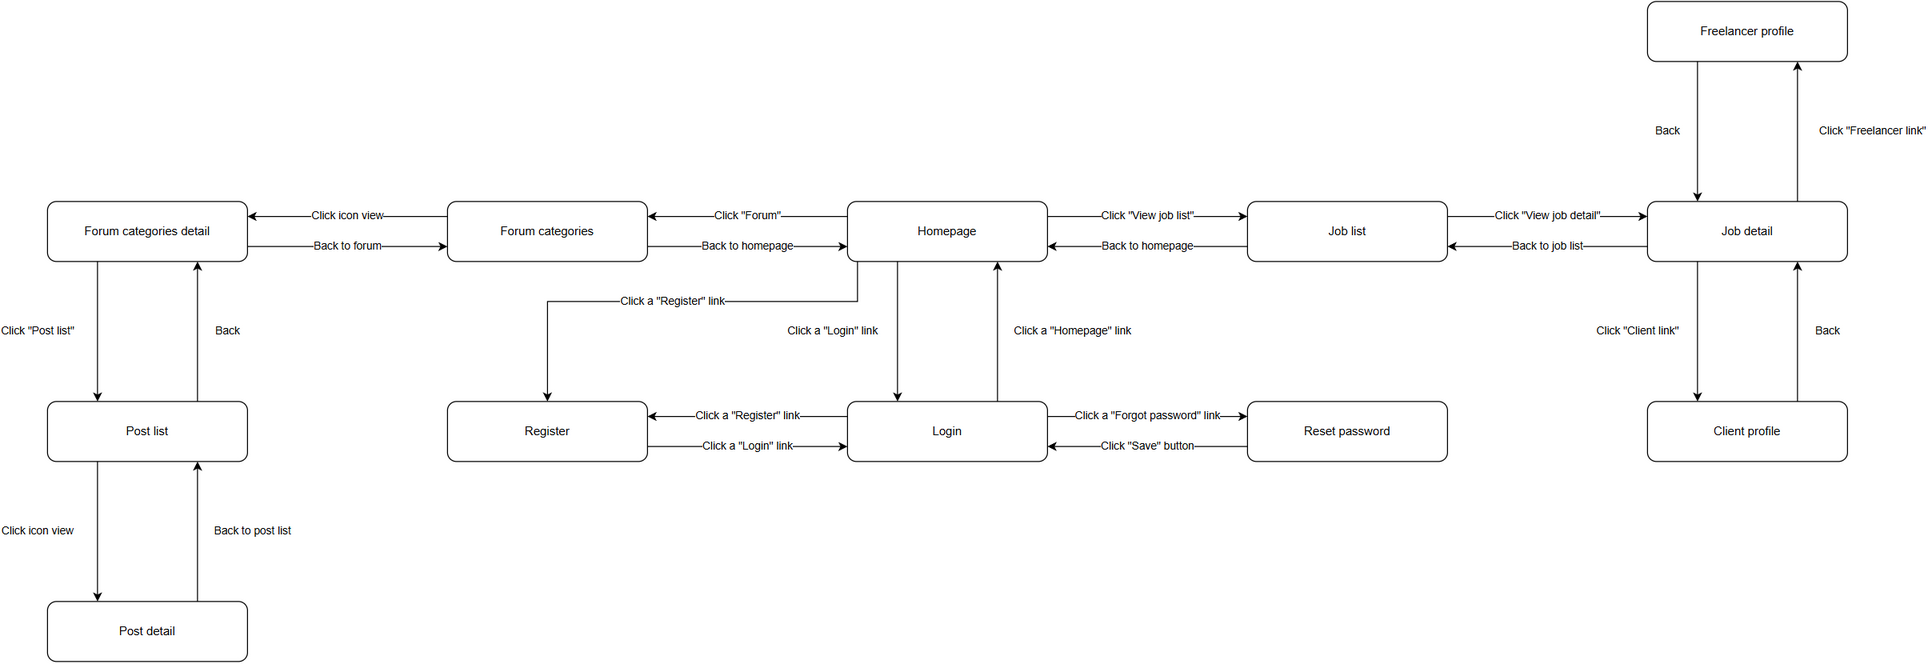
\includegraphics[width=\linewidth]{image/Screen_flow/Screen_flow_for_guest.drawio.png}
    \caption{Screen Flow of Guest}
    \label{fig:screenflowguest}
\end{figure}

\begin{figure}[H]
    \centering
    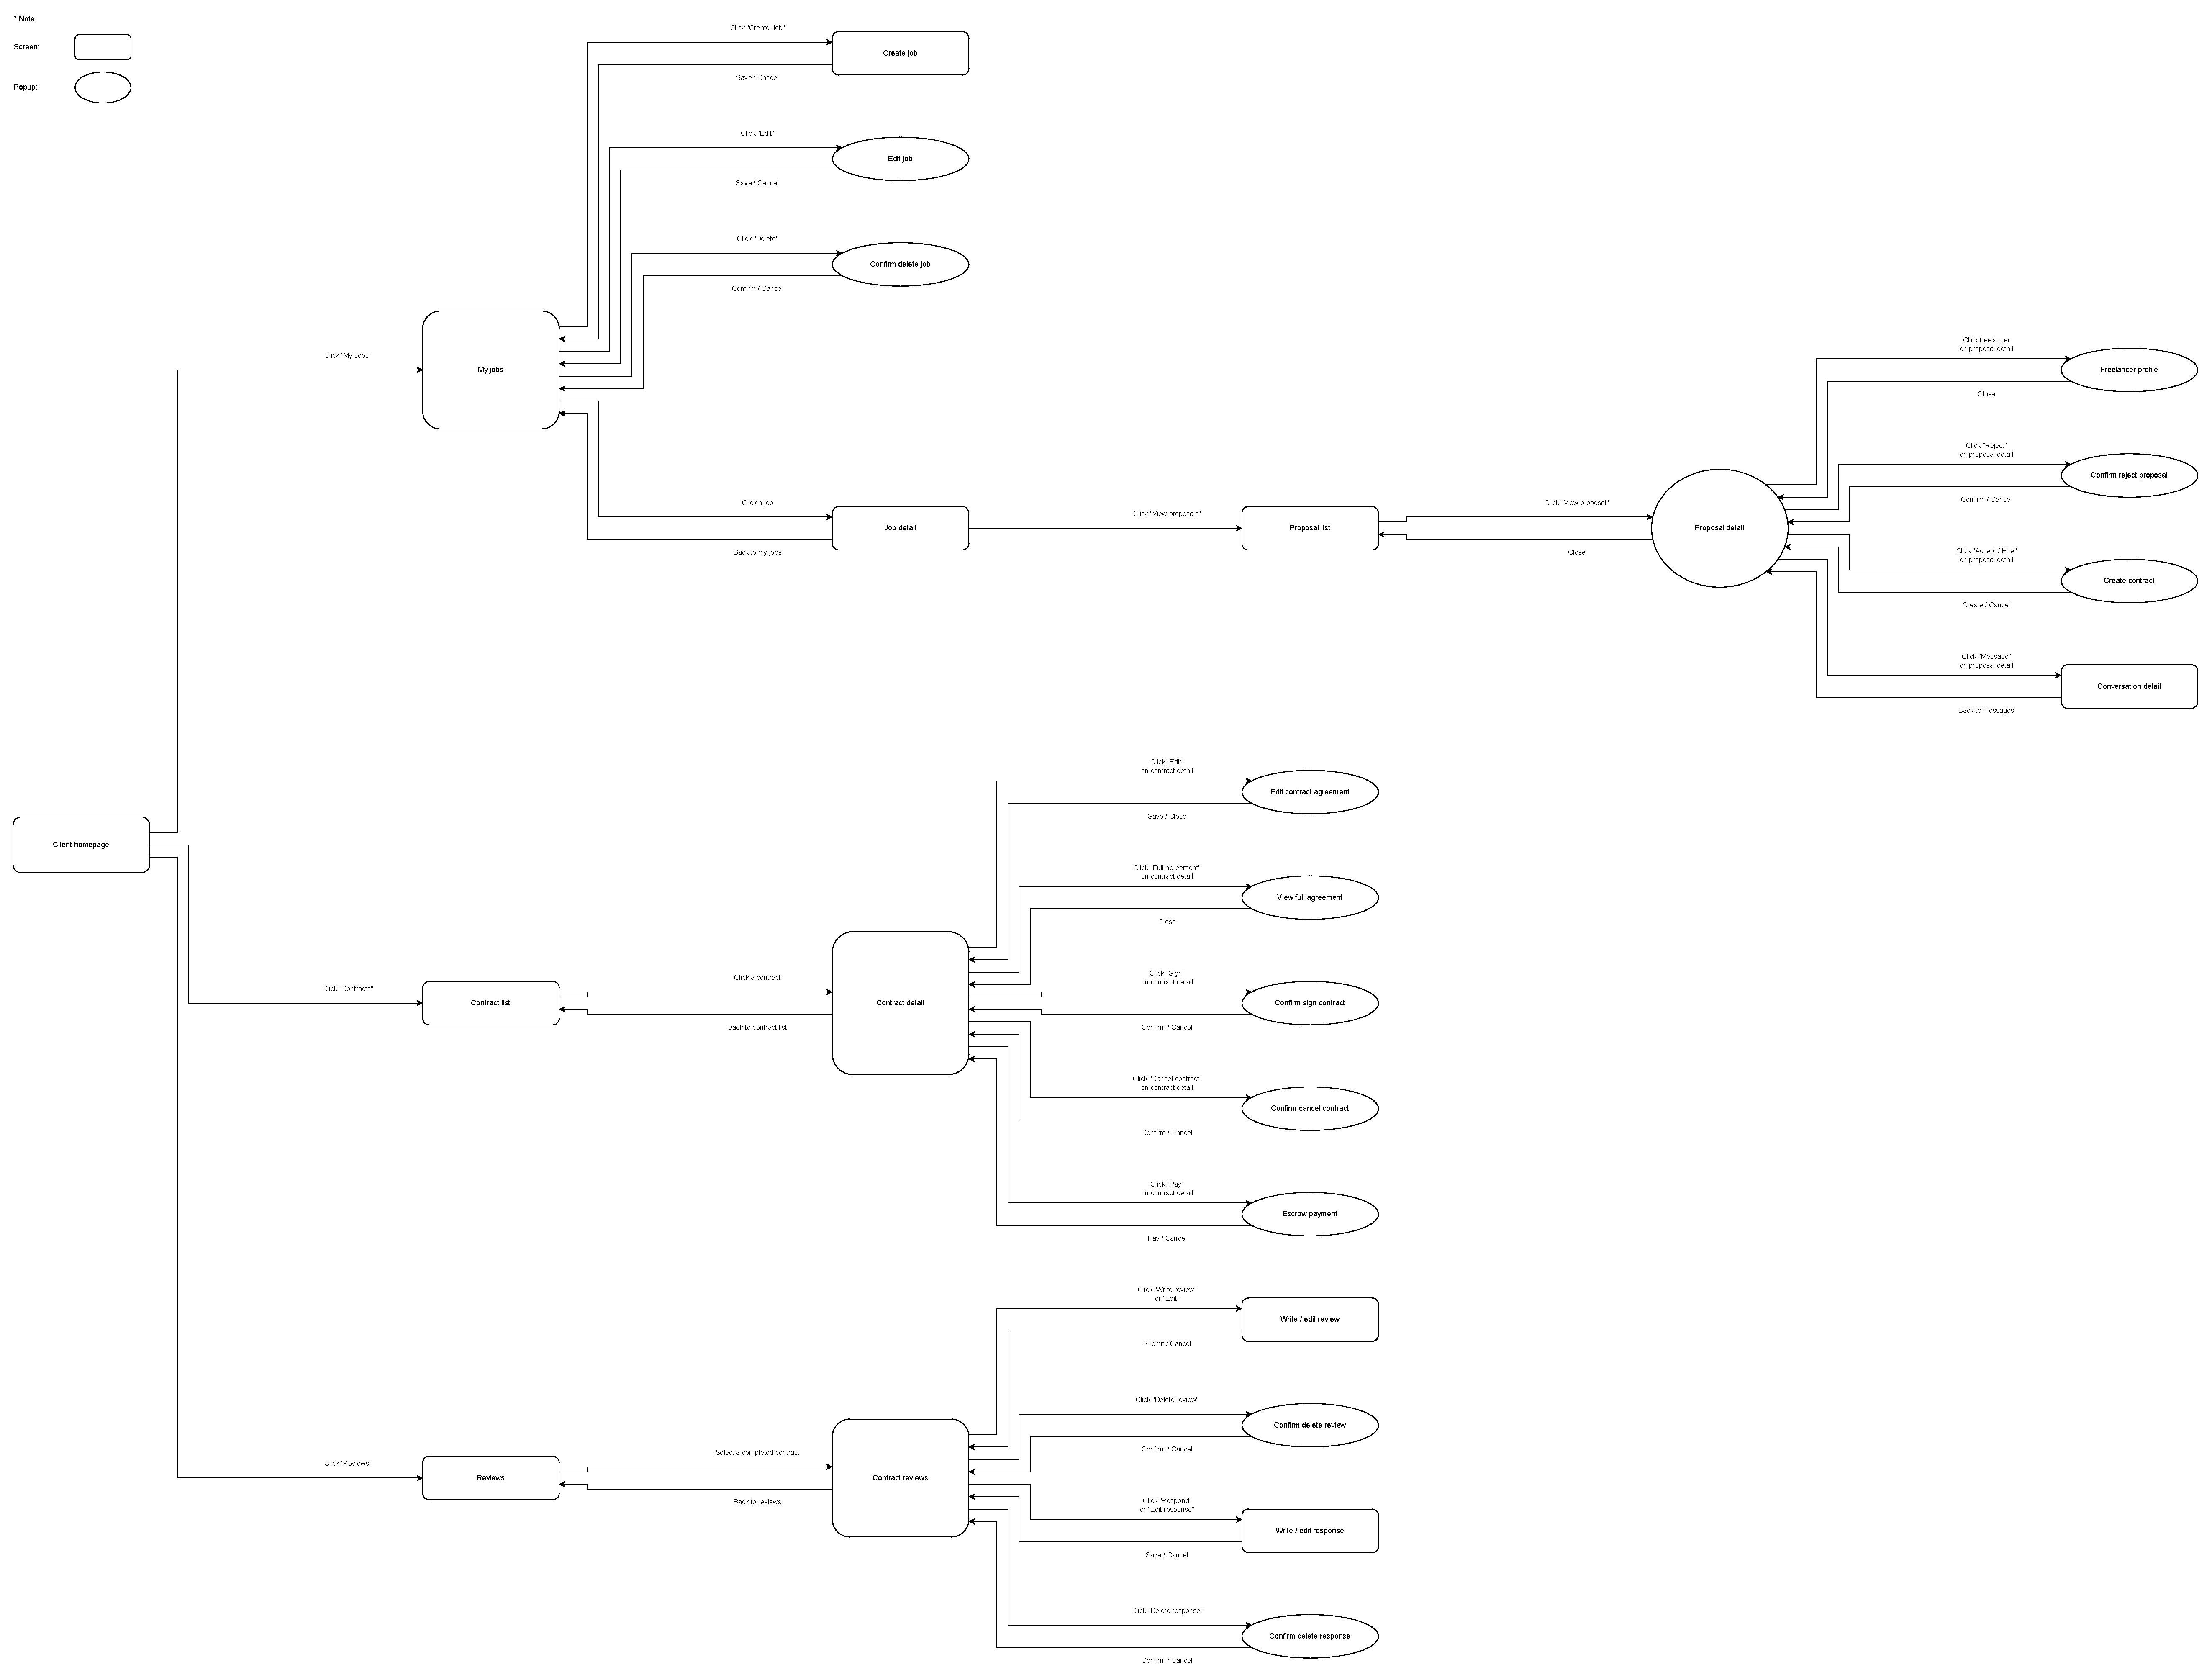
\includegraphics[width=\linewidth]{image/Screen_flow/Screen_flow_for_client_1.pdf}
    \caption{Screen Flow of Client (Part 1)}
    \label{fig:screenflowclient}
\end{figure}

\begin{figure}[H]
    \centering
    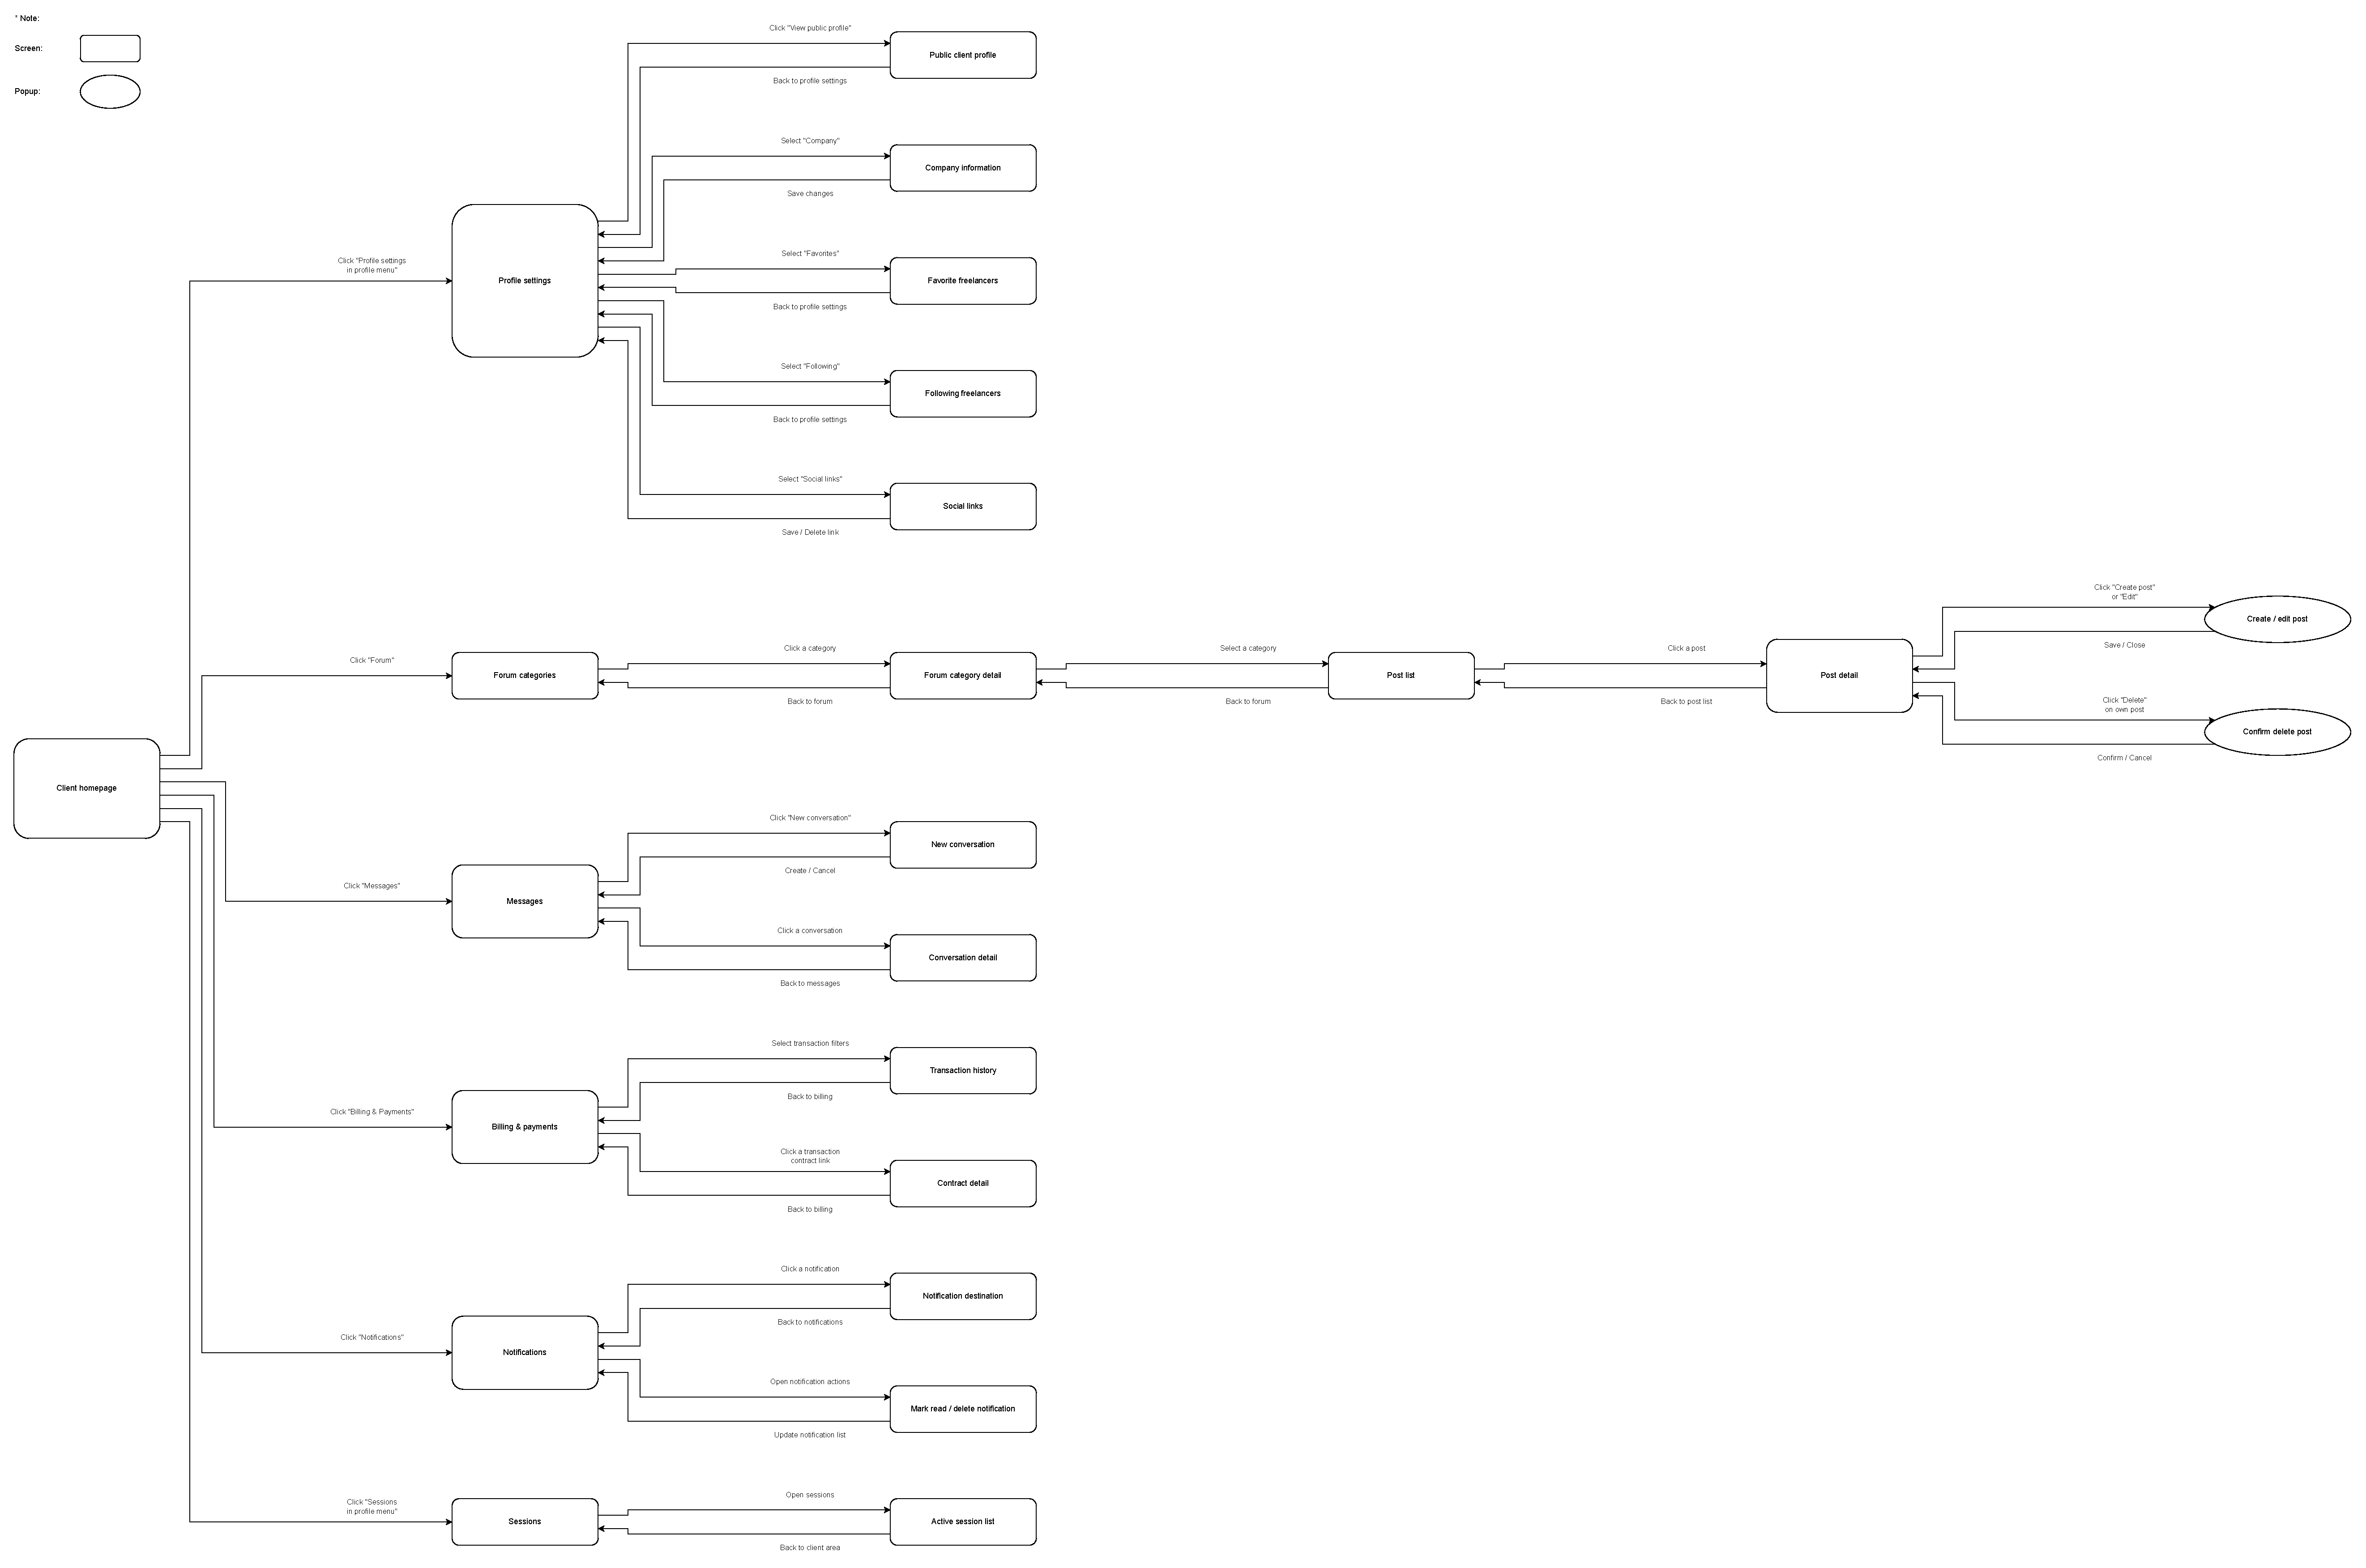
\includegraphics[width=\linewidth]{image/Screen_flow/Screen_flow_for_client_2.pdf}
    \caption{Screen Flow of Client (Part 2)}
    \label{fig:screenflowclient2}
\end{figure}

\begin{figure}[H]
    \centering
    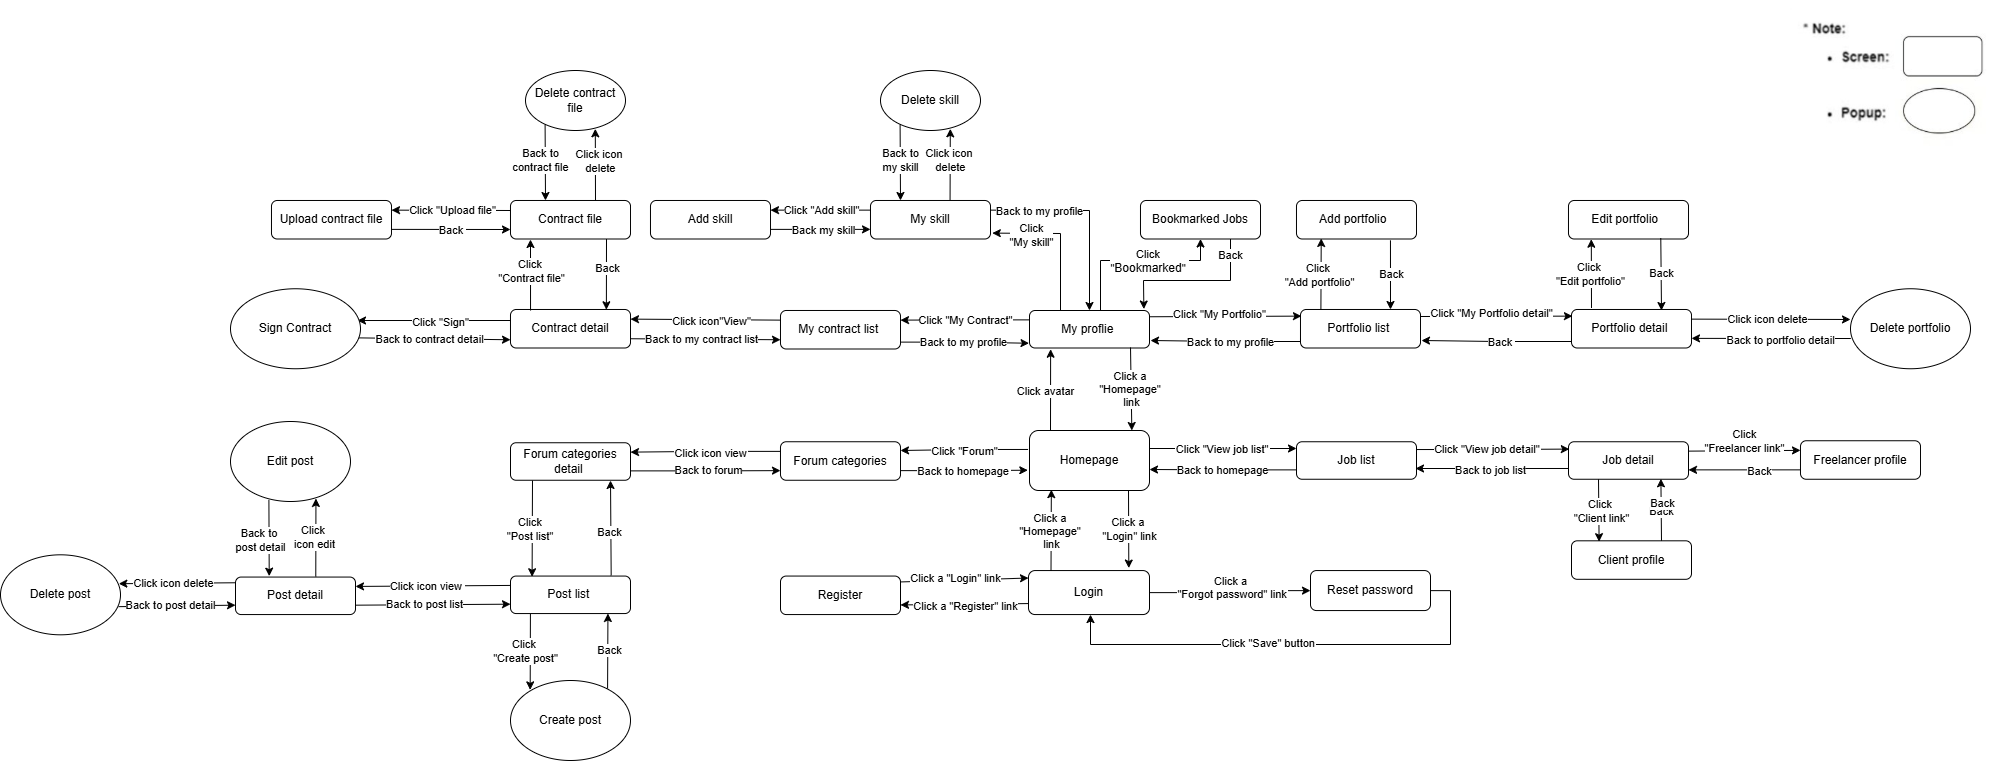
\includegraphics[width=\linewidth]{image/Screen_flow/Screen_flow_for_freelancer.drawio.png}
    \caption{Screen Flow of Freelancer}
    \label{fig:screenflowfreelancer}
\end{figure}

\begin{figure}[H]
    \centering
    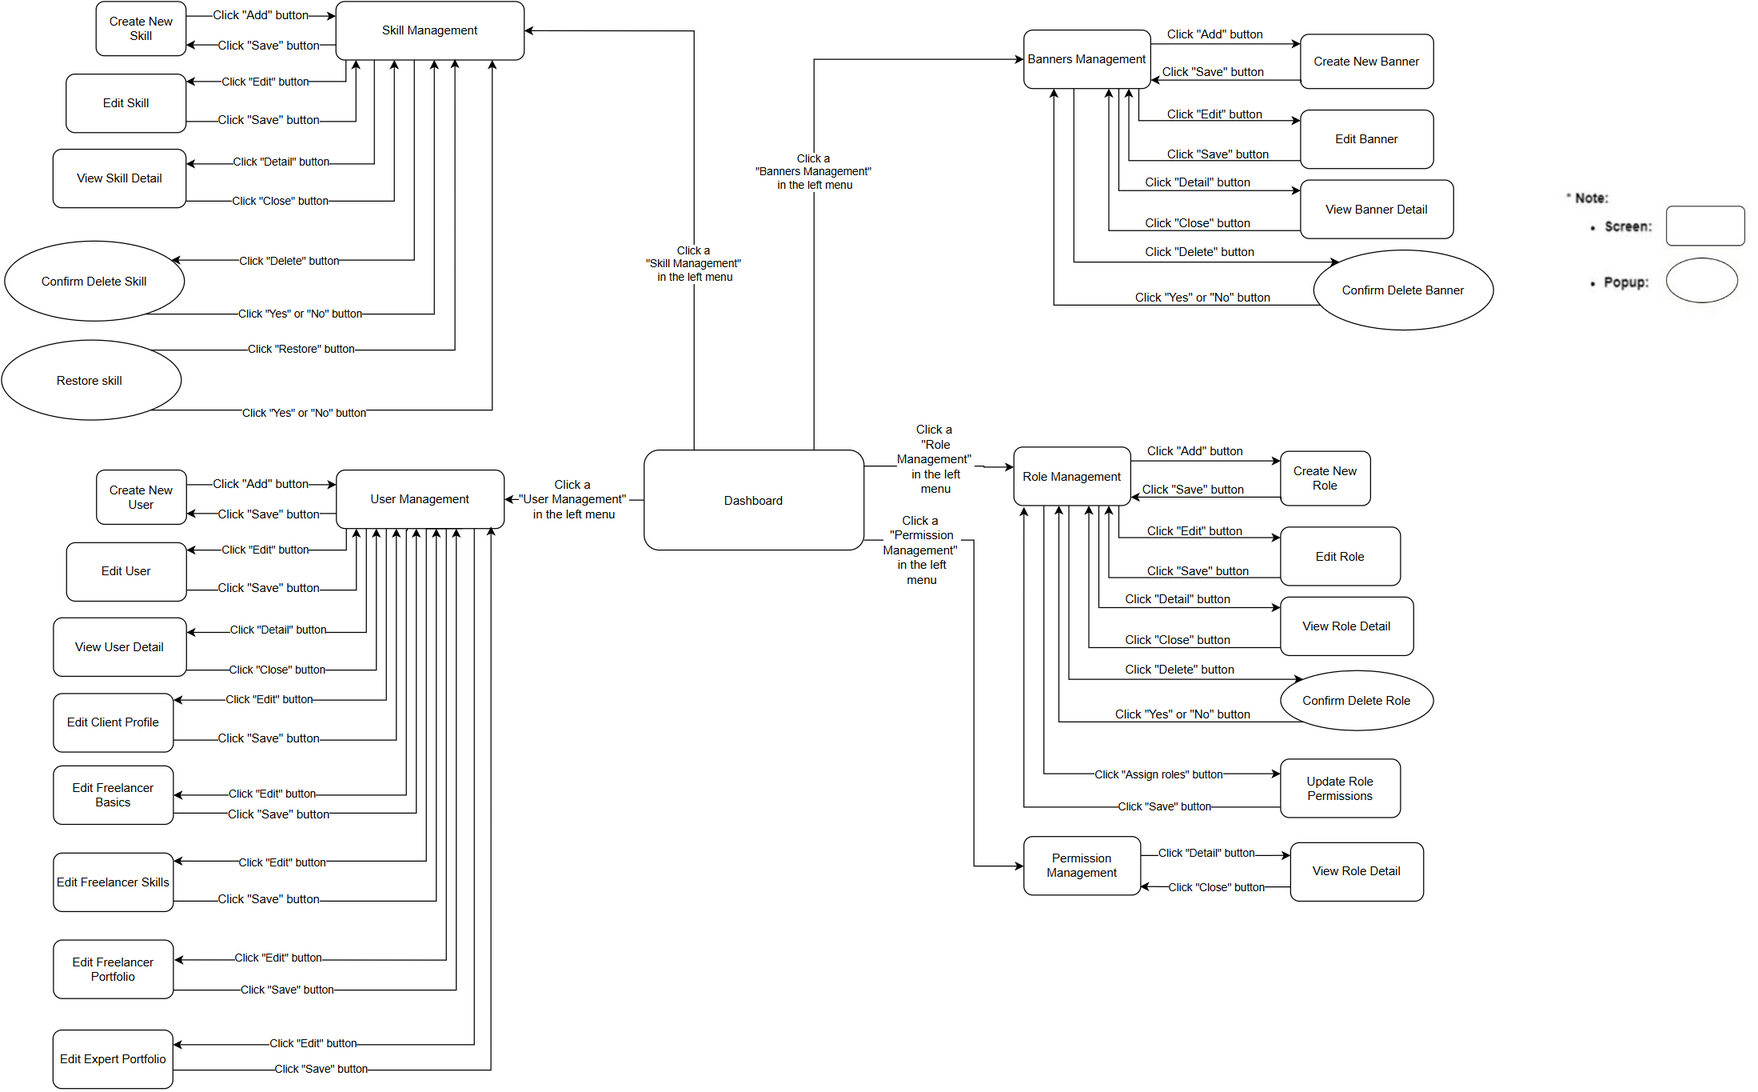
\includegraphics[width=\linewidth]{image/Screen_flow/Screen_flow_for_admin_1.drawio.png}
    \caption{Screen Flow of Admin (Part 1)}
    \label{fig:screenflowadmin1}
\end{figure}

\begin{figure}[H]
    \centering
    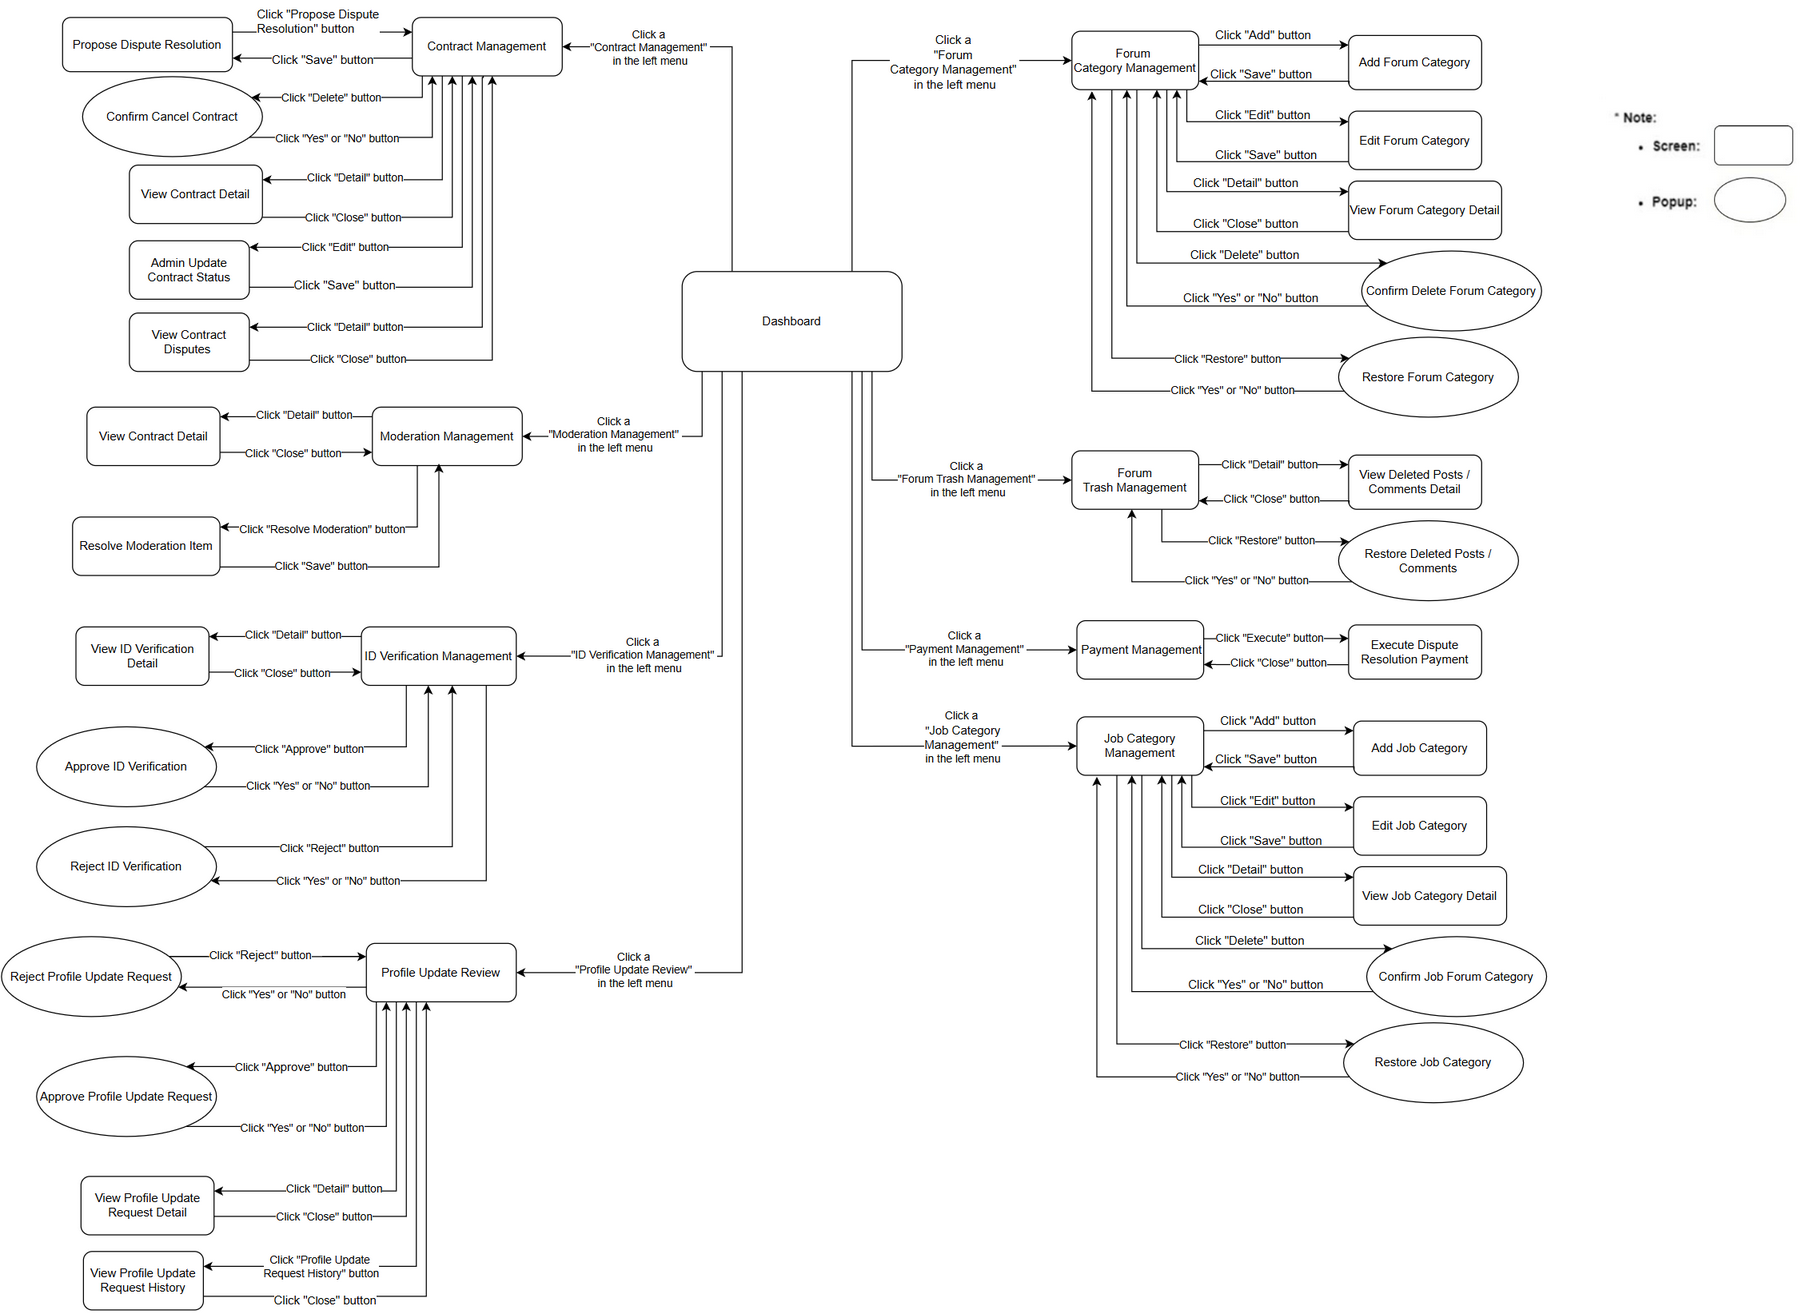
\includegraphics[width=\linewidth]{image/Screen_flow/Screen_flow_for_admin_2.drawio.png}
    \caption{Screen Flow of Admin (Part 2)}
    \label{fig:screenflowadmin2}
\end{figure}

% Ngắt trang bắt buộc để phần Bảng bên dưới sang trang mới sạch sẽ, không bị dính vào ảnh
\clearpage
